\documentclass[12pt]{article}

\usepackage{amsmath}
\usepackage{amsfonts}
\usepackage{float}
\usepackage{multicol}
\usepackage{fancyhdr}
\usepackage{graphicx}
\usepackage[colorlinks=true,linkcolor=blue, citecolor=red]{hyperref}
\usepackage{url}
\usepackage{parskip}
\usepackage[top=.75in, left=.5in, right=.5in, bottom=1in]{geometry}
\usepackage[utf8]{vietnam}
\setlength{\headheight}{29.43912pt}

% \graphicspath{PATH_TO_GRAPHIC_FOLDER}

\pagestyle{fancy}
\lhead{
\reportname
}
\rhead{
Trường Đại học Khoa học Tự nhiên - ĐHQG HCM\\
\coursename
}
\lfoot{\LaTeX\ by \href{https://github.com/trhgquan}{Quan, Tran Hoang}}

\newcommand{\coursename}{Mã hóa ứng dụng - CSC15003}
\newcommand{\reportname}{Trust Negotiation}
\newcommand{\trustx}{$\mathcal{\text{Trust-}X}$\ }

\begin{document}

\begin{titlepage}
\newcommand{\HRule}{\rule{\linewidth}{0.5mm}}
\centering

\textsc{\LARGE đại học quốc gia tphcm}\\[1.5cm]
\textsc{\Large trường đại học khoa học tự nhiên}\\[0.5cm]
\textsc{\large khoa công nghệ thông tin}\\[0.5cm]
\textsc{bộ môn công nghệ tri thức}\\[0.5cm]

\HRule \\[0.4cm]
{ 
\huge{\bfseries{Báo cáo Đồ án cuối kì}}\\[0.5cm]
\large{\bfseries{Đề tài: \reportname}}
}\\[0.4cm]
\HRule \\[0.5cm]

\textbf{\large Môn học: \coursename}\\[0.5cm]

\begin{minipage}[t]{0.4\textwidth}
\begin{flushleft} \large
\emph{Sinh viên thực hiện:}\\
Trần Hoàng Quân \textsc{(19120338)}\\
Lê Hoàng Trọng Tín \textsc{(19120682)}\\
Lê Mai Nguyên Thảo \textsc{(19120661)}
\end{flushleft}
\end{minipage}
~
\begin{minipage}[t]{0.4\textwidth}
\begin{flushright} \large
\emph{Giáo viên hướng dẫn:} \\
% Dr. James \textsc{Smith}
Thầy Trương Toàn Thịnh
\end{flushright}
\end{minipage}\\[2cm]

{\large \today}\\[2cm]


\includegraphics[scale=.25]{img/hcmus-logo.png}\\[1cm]

\vfill
\end{titlepage}
	
\tableofcontents
\pagebreak

\section{Trust Negotiation}
\subsection{Bài toán thực tế}
Xét qui trình thanh toán bằng thẻ tín dụng (hoặc thẻ NAPAS) ở siêu thị như sau:
\begin{enumerate}
\item Nhân viên thu ngân kiểm tra thẻ có hợp lệ hay không
\item Nhân viên thu ngân quẹt thẻ vào máy POS và cho khách hàng nhập mã PIN, số tiền.
\item Nhân viên thu ngân xác nhận thanh toán và in biên lai cho khách hàng ký.
\item Nhân viên thu ngân xác nhận chữ ký trên biên lai giống với chữ ký trên mặt sau của thẻ.
\end{enumerate}
Có thể nhận thấy, qui trình trên vẫn tiềm ẩn nhiều nguy cơ an ninh. Ví dụ, không phải ai cũng có kĩ năng chuyên môn để kiểm tra thẻ hợp lệ bằng mắt thường; không có gì đảm bảo nhân viên thu ngân không lợi dụng sơ hở của khách hàng để thay đổi số tiền, ..etc. Tuy tiềm ẩn nguy cơ, nhưng các giao dịch vẫn diễn ra hàng ngày vì sự tin tưởng của khách hàng với các tổ chức / nhãn hàng lớn.

Trên không gian số cũng vậy, phải có cách để tạo dựng sự tin cậy trong các giao dịch, các kết nối giữa các hệ thống với nhau. Đây cũng là lí do các giải pháp Trust Negotiation ra đời. Giống với thực tế, Trust Negotiation phải đạt được các mục tiêu sau:
\begin{itemize}
\item Tạo dựng sự tin cậy (Trust Establishment) giữa các bên tham gia.
\item Dù trao đổi các thông tin xác thực (credentials) với nhau, các thông tin này phải được giữ an toàn. 
\end{itemize}

\subsection{Trust Establishment (Thiết lập sự tin cậy)}
Mục tiêu của Trust Establishment là thiết lập sự tin cậy giữa những bên liên quan trong một hệ thống mở. Các bên này thường không cùng một miền bảo mật (security domain) với nhau, và do đó người ta thường không dùng danh tính (identity) mà dùng các thuộc tính (attributes) cho các thao tác xác thực sau này.

\subsection{Digital Credentials (Thông tin xác thực số)}
Digital Credentials chứa các thông tin dưới dạng thuôc tính của người / bên sở hữu và được cấp bởi một bên đáng tin cậy (thường là các ceritificate authority (CA) - nhà cung cấp chứng thư số).

Digital Credentials có các đặc điểm sau:
\begin{itemize}
\item Không thể làm giả.
\item Các thông tin được lưu trong Digital Credentials phải dễ xác thực.
\item Dùng PKI (public-key infrastructure, thường dùng chuẩn X.509 v3) để ký.
\end{itemize}

\subsection{Credential Disclosure Policy (CDP - Chính sách tiết lộ thông tin xác thực)}
Credential Disclosure Policy (CDP) là điều kiện đưa ra để một bên công bố các tài nguyên (resources) hoặc cho phép truy cập dịch vụ (services). Cần lưu ý là CDP áp dụng không chỉ cho resources và services. Vẫn có những policy áp dụng để bảo vệ credentials, kể cả CDP.

\subsection{Định nghĩa Trust Negotiation}
Trust Negotiation là phương pháp sử dụng cách tiếp cận kiểm soát truy cập (access control) và xác thực (authentication), cho phép bên yêu cầu tài nguyên (Resource Requester) và bên cung cấp tài nguyên (Provider) thiết lập sự tin cậy trên các hệ thống mở. Quá trình này dựa trên các thuộc tính (attributes) hơn là danh tính (identity).

Một số tính chất của Trust Negotiation:
\begin{itemize}
\item Trao đổi digital credentials môt cách tuần tự.
\item Mức độ nhạy cảm của credentials tăng dần khi độ tin cậy tăng dần.
\end{itemize}

\begin{figure}[H]
\centering
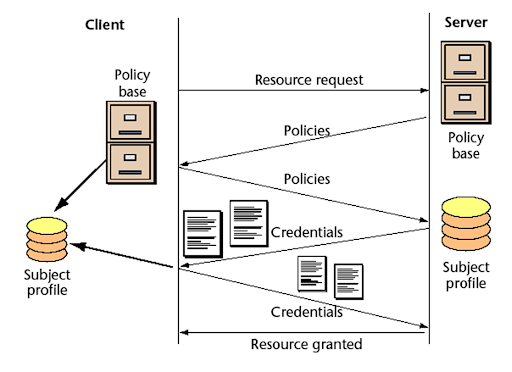
\includegraphics[scale=.5]{img/trust-simple.png}
\caption{Một mô hình Trust Negotiation đơn giản}
\label{fig:simple-trust}
\end{figure}

Các yêu cầu của một hệ thống Trust Management:
\begin{itemize}
\item Đảm bảo quyền sở hữu của credential.
\item Đảm bảo tính hợp lệ của credential.
\item Khám phá credential chain.
\item Có cơ chế bảo vệ quyền riêng tư.
\item Hỗ trợ các chiến thuật negotiate thay thế.
\begin{itemize}
\item Tăng cường bảo mật, tối ưu tính toán, ..etc
\end{itemize}
\item Các chiến thuật negotiate phải đảm bảo tốc độ (nhanh).
\end{itemize}

\section{Một số mô hình áp dụng Trust Negotiation}
Một số hệ thống Trust Management có thể kể đến:
\begin{itemize}
\item Keynote trust management system.
\item Trust Establishment phát triển bởi Haifa Research Lab.
\begin{itemize}
\item Trust Policy Language (TPL)\cite{848442}
\end{itemize}
\item TrustBuilder
\item Unipro
\item \trustx
\end{itemize}

Trong đó chúng ta đi sâu vào tìm hiểu các kiến trúc ATNAC và \trustx.

\subsection{ATNAC}
Adaptive Trust Negotiation and Access Control (ATNAC)\cite{10.1145/1063979.1064004}, là kiến trúc access control được ứng dụng vào các dịch vụ điện tử, sử dụng các hệ thống TrustBuilder và GAA-API. 

\subsubsection{TrustBuilder}
Được phát triển bởi Đại học Brigham Young (BYU) và Đại học Illinois Urbana-Champaign (UIUC). Hệ thống chỉ thực hiên qui trình Trust Negotiation, tuy nhiên có nhiều khuyết điểm:
\begin{itemize}
\item Dễ bị tấn công DoS (denial of service - tấn công từ chối dịch vụ).
\begin{itemize}
\item Attacker gửi số lượng lớn sessions lên server khiến hệ thống bị nghẽn.
\item Các policy có chi phí tính toán phức tạp, tốn nhiều thời gian tính toán.
\item Tính toán và xác thực các credentials không hợp lệ hoặc không liên quan gây lãng phí. 
\end{itemize}
\item Các cuộc tấn công vào hê thống TrustBuilder thường nhắm vào các thông tin nhạy cảm.
\end{itemize}
Để khắc phục khuyết điểm này, ATNAC sử dụng middleware GAA-API.

\subsubsection{GAA-API}
Generic Authorization and Access-control API (GAA-API) là một middleware API, sử dụng cơ chế FGAC (Fine-grained access control - kiểm soát truy cập chi tiết). GAA-API có thể phát hiện và phản hồi lại các cuộc xâm nhập ở mức ứng dụng, có thể tương tác với các hệ thống IDS (Intrusion Detection System - hệ thống phát hiện xâm nhập) để thích ứng với các điều kiện đe dọa mạng.

Cần lưu ý, GAA-API chỉ đóng vai trò kiểm soát truy cập, không tham gia vào quá trình Trust Negotiation.

\begin{figure}[H]
\centering
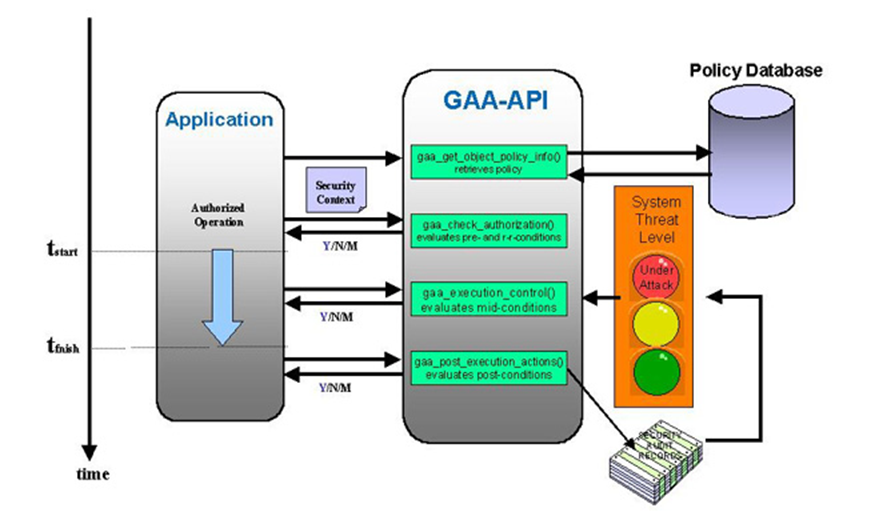
\includegraphics[scale=.5]{img/gaa-api.png}
\caption{Sơ đồ hoạt động của GAA-API}
\label{fig:gaa-api}
\end{figure}

\subsubsection{Suspicion Level}
Suspicion Level đánh giá khả năng Requester đang thực hiên hành động không phù hợp, gồm ba yếu tố chính:
\begin{itemize}
\item $S_{DOS}$: Khả năng Requester đang thực hiện tấn công DoS.
\item $S_{IL}$: Khả năng Requester đang cố gắng làm rò ri thông tin (information leakage).
\item $S_{O}$: Các hành vi đáng ngờ khác.
\end{itemize}

Mỗi Requester có một Suspicion Level riêng. Suspicion Level tăng khi một sự kiện được đánh giá là "đáng ngờ" xảy ra, giảm khi các sự kiện được đánh giá là "tích cưc" xảy ra. Cụ thể:

\begin{itemize}
\item Analyzer của GAA-API xác định các Requesters gửi một số lượng lớn request có sự tương đồng bất thường, sau đó tăng $S_{DOS}$.
\item Trong quá trình Trust Negotiation, nếu các credentials client gửi lên hệ thống không trùng với credentials hệ thống yếu cầu, $S_{DOS} = 1$.
\item Nếu $S_{DOS}, S_{IL}$ hoặc $S_O > 0.9$, hệ thống sẽ kích hoạt firewall chặn Requester.
\item Nếu $S_{IL} > threshold$, nghĩa là vượt quá ngưỡng $threshold$ nhất định, hệ thống sẽ xác định người dùng đang có ý định làm rò rỉ thông tin và sẽ áp dụng các policy nghiêm ngặt hơn với credentials. Tổng quát, $S_{IL}$ càng tăng thì các Access Control Policies được áp dụng sẽ càng chặt hơn.
\end{itemize}

Một ví dụ cụ thể:

\begin{figure}[H]
\centering
\begin{multicols}{2}
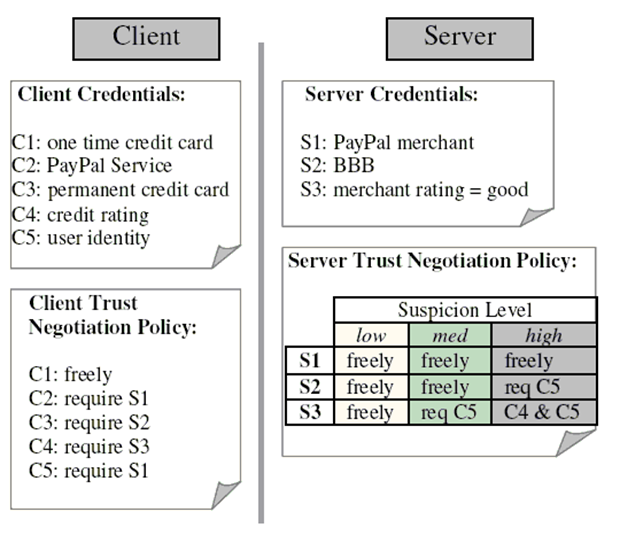
\includegraphics[scale=.5]{img/atnac-example-1.png}

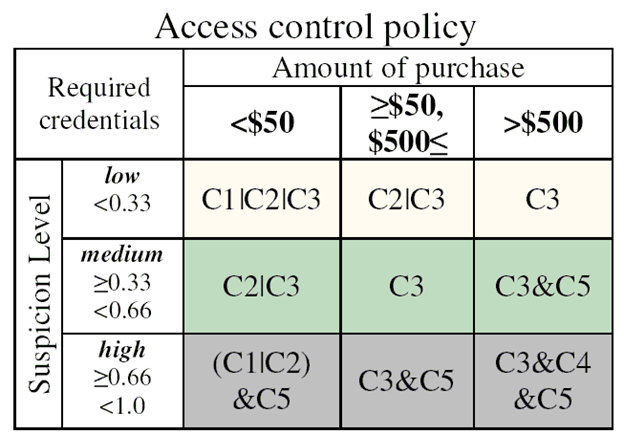
\includegraphics[scale=.5]{img/atnac-example-2.png}
\end{multicols}
\caption{Credentials, Policies và Access Control Policy của một trang thương mại điện tử.}
\end{figure}

Xét trường hợp khách hàng muốn mua món đồ với giá > \$500. Khi đó:
\begin{itemize}
\item Nếu Suspicion Level ở mức low, policy chỉ yêu cầu credential C3.
\item Nếu Suspicion Level ở mức medium, policy yêu cầu credential C3 và C4.
\item Nếu Suspicion Level ở mức high, policy yêu cầu cung cấp credential C3, C4 và C5.
\end{itemize}
Có thể thấy, Suspicion Level càng cao thì policy áp dụng lên càng phức tạp.

\subsubsection{Mô hình ATNAC}
ATNAC kết hợp hai hệ thống TrustBuilder và GAA-API để bổ sung khuyết điêm của mỗi hệ thống. Khi đó, chi phí tính toán của quá trình Trust Negotiation sẽ được tối ưu, hạn chế các cuộc tấn công vào hệ thống. ATNAC cũng sẽ hỗ trợ các chính sách thích ứng chi tiết. Kiến trúc cụ thể của ATNAC như hình dưới:

\begin{figure}[H]
\centering
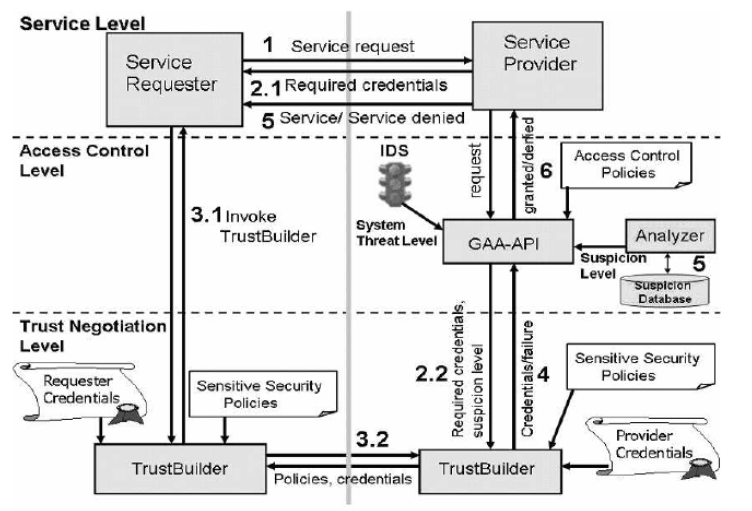
\includegraphics[scale=.7]{img/atnac.png}
\caption{Kiến trúc mô hình ATNAC}
\end{figure}
Một session thể hiện quá trình Trust Negotiation sẽ gồm các giai đoạn:
\begin{itemize}
\item Service Requester gửi service request lên Service Provider (1), Provider sau đó chuyển cho GAA-API xử lí. API sẽ đánh giá các access control policies kiểm soát quyền truy cập của service đó. Các policies sau đó cũng đưa ra danh sách các credentials cần thiết để thỏa yêu cầu, các credentials này còn tùy thuộc vào độ nhạy cảm, mức độ đe dọa (threat level) và suspicion level của Requester.
\item GAA-API sẽ dùng các credentials này để đánh giá và đưa ra quyết định chấp nhận hay từ chối request (6). Trường hợp credential chưa có hoặc threat level quá cao, API sẽ yêu cầu Requester cung cấp thêm credentials (2.1). Cùng lúc đó, Analyzer sẽ tính toán Suspicion Level của Requester, sau đó GAA-API chuyển danh sách credentials và Suspicion Level cho TrustBuilder (2.2).
\item Requester nhận yêu cầu cung cấp thêm credentials (2.1) và bắt đầu giai đoạn Trust Negotiation (3.1) với TrustBuilder server. Server và client sẽ giao tiếp liên tục để nhận về credentials đã yêu cầu (3.2). Cũng trong quá trình này, TrustBuilder dựa vào Suspicion Level để đưa ra các Credential Release Policy phù hợp. Nếu các policies của TrustBuilder đều thỏa mãn và các credentials client cung cấp đều hợp lệ, bước Negotiation đã thành công, credentials được trả về GAA-API (4).
\item GAA-API dùng kết quả từ Trust Negotiation (4) để đánh giá nên cấp quyền truy cập hay từ chối yêu cầu truy cập service (6).
\item (5): Analyzer lưu lại thông tin các Requester có hành vi đáng ngờ vào Suspicion Database để tiện truy xuất.
\end{itemize}

\subsubsection{Tổng kết}
Một số đặc điểm của mô hình ATNAC có thể kể đến như:
\begin{itemize}
\item Hạn chế các cuộc tấn công DoS, gây rò rỉ dữ liệu.
\item Linh hoạt áp dụng các policies đối với từng đối tượng ở các mức Suspicion Level khác nhau.
\end{itemize}
Một số nhược điểm của ATNAC có thể kể đến:
\begin{itemize}
\item Số lượng policy áp dụng có thể tăng dần khi Suspision Level tăng, số luợng credentials có thể nhiều hơn mức bình thường cho quá trình negotiation.
\end{itemize}

\subsection{\trustx}
\trustx\cite{10.1109/TKDE.2004.1318565} là một kiến trúc thiết kế riêng cho môi trường P2P (Peer-to-Peer), trong đó các bên có thể vừa đống vai trò là Requester hoăc Controller. Hệ thống thiết kế dựa trên nền XML, sử dụng ngôn ngữ X-TNL để đặc tả các policies và certificates. 

\begin{figure}[H]
\centering
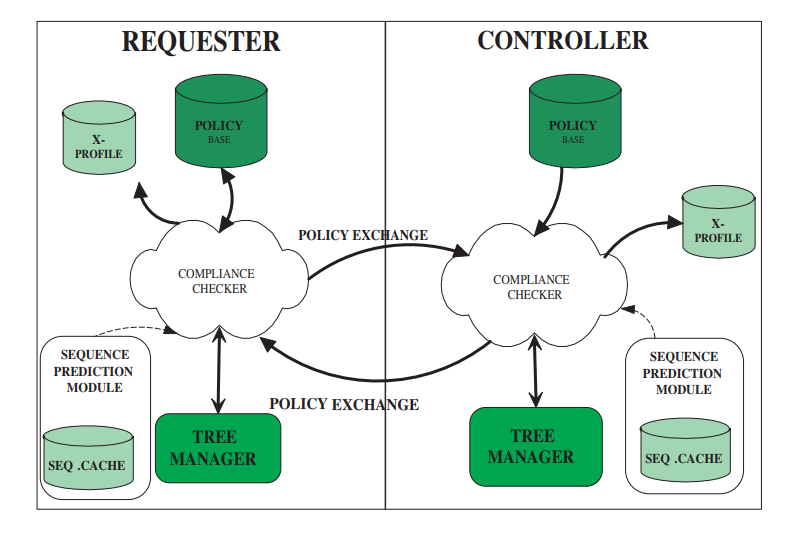
\includegraphics[scale=.8]{img/trust-x-architecture.png}
\caption{Sơ đồ (đơn giản) mô hình \trustx}
\end{figure}

Mô hình có các đặc điểm đáng chú ý sau:

\subsubsection{Certificates}
Tương ứng với credentials của ATNAC, nhưng gồm hai loại:
\begin{itemize}
\item Credentials: Mang các thuộc tính của chủ sở hữu, được công nhận bởi CA.
\item Declarations: Mang các thông tin của chủ sỡ hữu, không cần công nhận.
\end{itemize}

\begin{figure}[H]
\centering
\begin{multicols}{2}
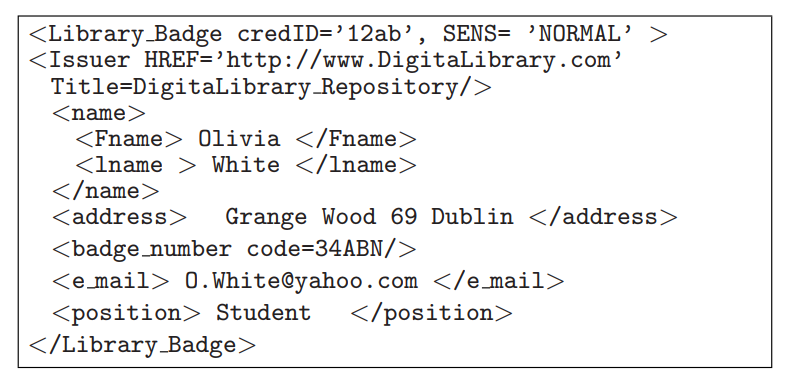
\includegraphics[scale=.5]{img/trustx-credential.PNG}

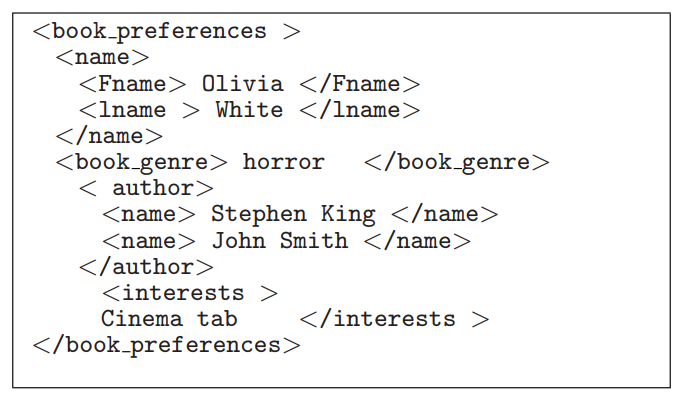
\includegraphics[scale=.5]{img/trustx-declaration.PNG}
\end{multicols}
\caption{Cấu trúc XML của credential (trái) và declaration (phải) certificate}
\end{figure}

\subsubsection{Các phase}
\trustx có ba phase:
\begin{itemize}
\item Introduction phase: trao đổi bằng các thông điệp ngắn, quy định bởi các chính sách giới thiệu (introductory policies) của hai bên. Mục tiêu của phase là xác định các thuôc tính cần thiết cho các bước negotiate tiếp theo.
\item Policy Evaluation phase: trao đổi các chính sách tiết lộ (disclosure policies) áp dụng cho các resources liên quan. Phase này thực hiện ở Compliance Checker. Quan trọng là phase \textbf{chỉ trao đổi các policies}, \textbf{không trao đổi các certificate}. Mục tiêu của phase là xác định chuỗi các certificates phù hợp với disclosure policies của cả server và client khi release resource.
\item Certificate Exchange phase: các bên công bố các certificate của mình, bên còn lại xác minh, tuần tự theo thứ tự đã có ở Policy Exchange phase. Resource được release khi không có vấn đề xảy ra.
\end{itemize}

\begin{figure}[H]
\centering
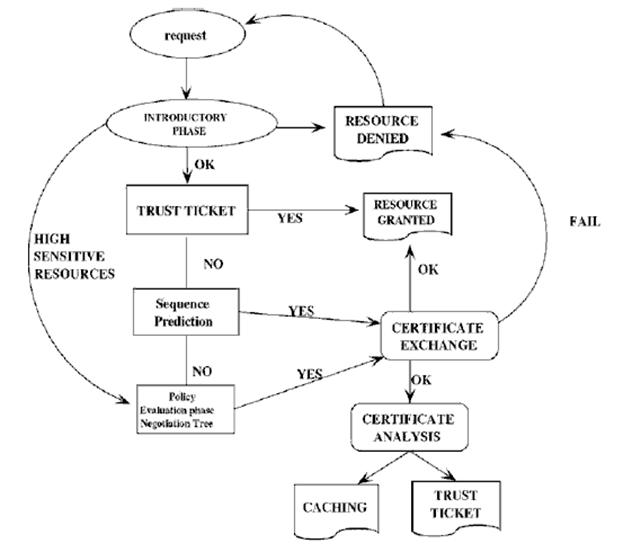
\includegraphics[scale=.8]{img/trustx-architecture.png}
\caption{Flowchart quá trình negotiation ở mô hình \trustx}
\end{figure}

Các module Trust Ticker, Sequence Prediction nhằm làm tăng tốc quá trình. Các policies được lưu trong một cấu trúc dữ liệu cây nhằm làm tăng tốc quá trình tìm kiếm và cập nhật.

\subsubsection{Tổng kết}
Một số đặc điểm của mô hình \trustx có thể kể đến:
\begin{itemize}
\item Tốc độ nhanh
\item Phân biệt riêng các phase trao đổi policy và certificate, từ đó không yêu cầu client cung cấp thêm thông tin như ATNAC.
\end{itemize}
Song song với đó là một số nhược điểm
\begin{itemize}
\item Lưu certificates dưới dạng XML, thân thiện với con người nhưng đôi khi có thể gây tác dụng ngược (rò rỉ thông tin, thông tin lại dễ đọc).
\end{itemize}

\section{Tổng kết}
Có nhiều mô hình ứng dụng Trust Negotiation, trong đó đặc biệt là các mô hình ATNAC (ứng dụng TrustBuilder) và \trustx. Mỗi mô hình có các ưu khuyết điểm riêng, từ đó phải cân nhắc sử dụng trong từng môi trường, đặc tính kĩ thuật khác nhau.

\addcontentsline{toc}{section}{Tài liệu}
\bibliographystyle{plain}
\bibliography{sample}

\end{document}